\documentclass{beamer}

\usepackage{booktabs}
\usepackage{braket}
\usepackage{calc}
\usepackage{listings}
\usepackage{mathtools}
\usepackage{soul}
\usepackage[uline]{hhtensor}
\newcommand{\eps}{\epsilon}
\newcommand{\EE}{\mathbb{E}}
\newcommand{\PP}{\mathbb{P}}
\newcommand{\RR}{\mathbb{R}}
\newcommand{\cE}{\mathcal{E}}
\newcommand{\cL}{\mathcal{L}}
\newcommand{\cO}{\mathcal{O}}
\newcommand{\cQ}{\mathcal{Q}}
\newcommand{\cS}{\mathcal{S}}
\newcommand{\KLD}[2]{D_{\mathrm{KL}}\left( #1||#2\right)}

\setbeamerfont{footnote}{size=\tiny}
\newtheorem{proposition}[theorem]{Proposition}
\newtheorem{remark}[theorem]{Remark}

\title{Fat-tailed variational inference}
\author{Feynman Liang, Liam Hodgkinson, Michael Mahoney}
\institute{UC Berkeley}
\date{\today}

\begin{document}

\frame{\titlepage}

\begin{frame}
    \frametitle{Motivating example}

    \begin{description}[leftmargin=!,labelwidth=\widthof{\bfseries b}]
        \item[Linear regression] $y = X \beta + \eps$, $\beta \in \RR^d$, $\eps\sim N(0,\sigma)$

        \item[Robust regression] $y = X \beta + \eps$, $\beta \in \RR^d$, $\eps\sim StudentT(\sigma)$

        \item[Bayesian robust regression] $y = X \beta + \eps$, $\beta \sim P$\;, $\eps\sim StudentT(\sigma)$
    \end{description}

    \begin{center}
        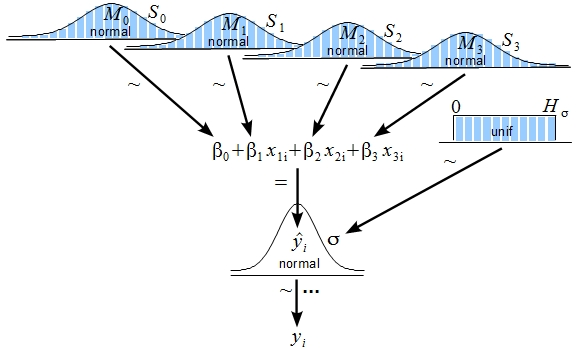
\includegraphics[width=0.6\textwidth]{Figures/bmlr.jpg}
        \footnote{https://jkkweb.sitehost.iu.edu/BMLR/}
    \end{center}
    \textbf{Goal}: approximate (observables of) $\PP(\beta \mid X, y)$

    % Robust means different things, could be robust objective / huber loss
    % Can we make it broad, but precisely this is the Bayesian / BDA notion of robust regression
\end{frame}

\begin{frame}
    \frametitle{Motivating example}

    \textbf{Goal}: approximate (observables of) $\PP(\beta \mid X, y)$

    \textbf{General solutions}:
    \begin{itemize}
        \item (MCMC, see LIC talk) sample $\beta_i \sim \PP(\beta \mid X, y)$:
              \[
                  n^{-1} \sum_i^n f(\beta_i) \to \EE_{\beta \mid X, y} f(\beta)
                  \qquad \forall f \in C(\RR^d)
              \]
        \item (Today's talk) search for variational approximation
              $q_{\theta^*} \in \cQ = \{q_\theta : \theta \in \Theta\}$
              ``close'' to $\PP(\beta \mid X, y)$
    \end{itemize}

    % Say we're interested in a general thing earlier, makes PPL transition easier
\end{frame}

\begin{frame}[allowframebreaks]
    \frametitle{Variational inference}

    \begin{definition}
        The \emph{forward KL Divergence}
        $\KLD{P}{q_\theta} = \EE_P \log \frac{\PP(\beta \mid X, y)}{q_\theta(\beta)}$,
        and the \emph{reverse KL Divergence} is $\KLD{q_\theta}{P}$.
    \end{definition}

    \begin{center}
        % \includegraphics[width=0.4\textwidth]{Figures/forward_kl_bad.png}
        % \includegraphics[width=0.4\textwidth]{Figures/forward_kl_good.png}
        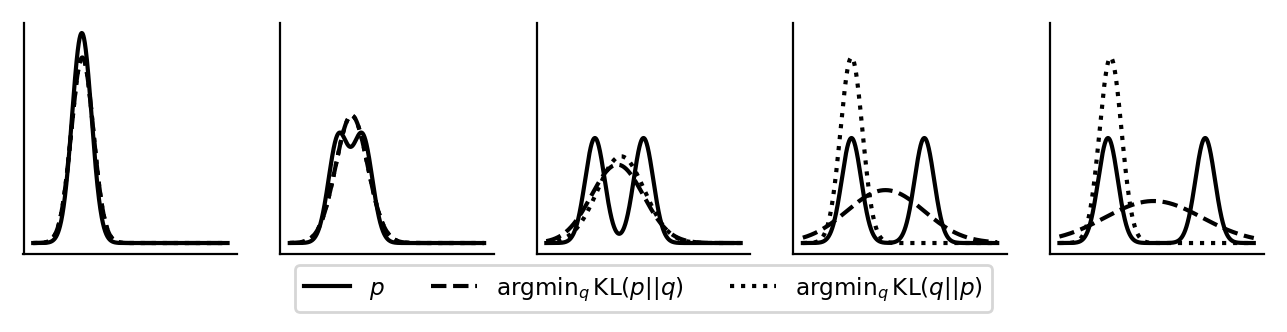
\includegraphics[width=0.9\textwidth]{Figures/reverse_forward_kl.png}
        \footnote{https://www.tuananhle.co.uk/notes/reverse-forward-kl.html}
    \end{center}

    \begin{itemize}
        \item Forward KL is mass-covering/mean-seeking,
              requires sampling/integrating $P$,
              density estimation objective
        \item Reverse KL is zero-forcing/mode-seeking,
              requires sampling/integrating $Q$,
              variational inference objective
    \end{itemize}

    \framebreak

    Evaluating $\PP(\beta \mid X, y) = \frac{\PP(\beta, X, y)}{\int \PP(\beta, X, y) d\beta}$ intractable!

    \begin{definition}
        The \emph{evidence lower bound}
        $ELBO(\theta) \coloneqq \EE_{q_\theta} \log \frac{\PP(\beta, X, y)}{q_\theta(\beta)}$.
    \end{definition}

    Can show $\KLD{q_\theta}{P} = \text{constant} - ELBO(\theta)$, so VI transforms
    (intractable) inference problem to a (tractable) optimization of an approximation:
    \[
        \PP(\beta \mid X, y) \approx \arg\max_{q_\theta \in \cQ} ELBO(\theta)
    \]
\end{frame}

\begin{frame}[allowframebreaks]
    \frametitle{Automatic differentiation variational inference (ADVI)}

    \begin{definition}[\footnote{Kucukelbir et al. ``Automatic differentiation variational inference.'' JMLR 2017}]
        \begin{align*}
            \cQ_{ADVI} = \{ q_\theta(\beta) =
            f_\ast N(\beta \mid \theta_{0}, e^{-\theta_{1}}) :
            \theta_0, \theta_1 \in \RR^d
            \}
        \end{align*}
        $f$ is a deterministic bijection between supports.
    \end{definition}

    \begin{center}
        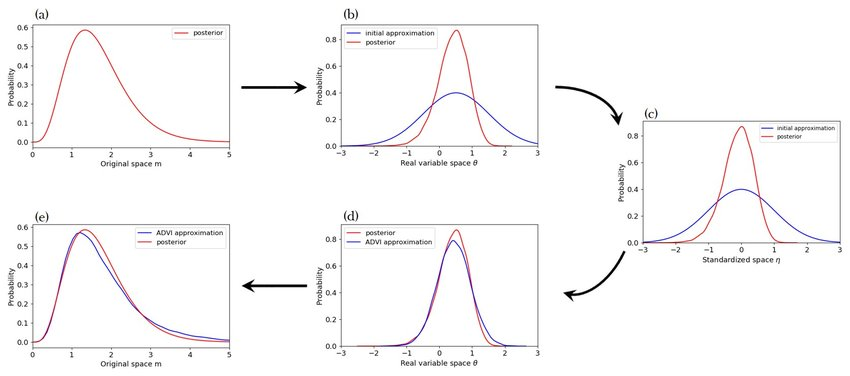
\includegraphics[width=0.8\textwidth]{Figures/advi.png}
        \footnote{Zhang, Xin, and Andrew Curtis. "Seismic tomography using variational inference methods." Journal of Geophysical Research: Solid Earth 125.4 (2020)}
    \end{center}

    \framebreak

    \textbf{Problem}: Gaussian approximations are too limited!

    \begin{center}
        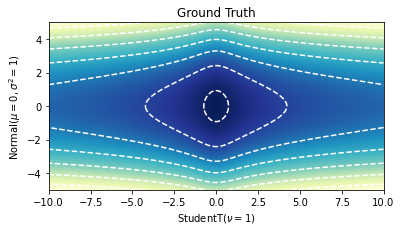
\includegraphics[width=0.45\textwidth]{../Figures/pancake-truth.png}
        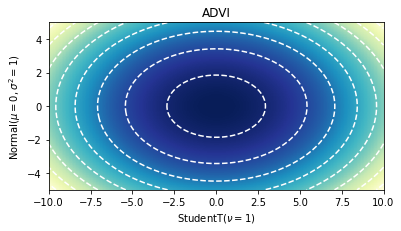
\includegraphics[width=0.45\textwidth]{../Figures/pancake-advi.png}
    \end{center}
\end{frame}

\begin{frame}[allowframebreaks]
    \frametitle{Normalizing flows}

    \textbf{Normalizing flows}: $f = f^{W}$ is a \st{deterministic} learnable bijection
    represented with neural networks.

    \begin{lemma}[Change of variable]
        If $Y = f(X)$ is an injective pushforward, then
        \[
            p_Y(y) = p_X(f^{-1}(y)) \lvert \det D f^{-1}(y) \rvert
        \]
    \end{lemma}

    Desiderata:
    \begin{itemize}
        \item Sampling: fast evaluation of $f$
        \item Density: fast evaluation of $f^{-1}$ and $\det D f$
    \end{itemize}

    \framebreak

    \begin{example}[Neural autoregressive flows]
        $y_i = \text{DNN}(x_t; W=c(x_{1:t-1}))$
        constrained strictly monotonic
        \begin{center}
            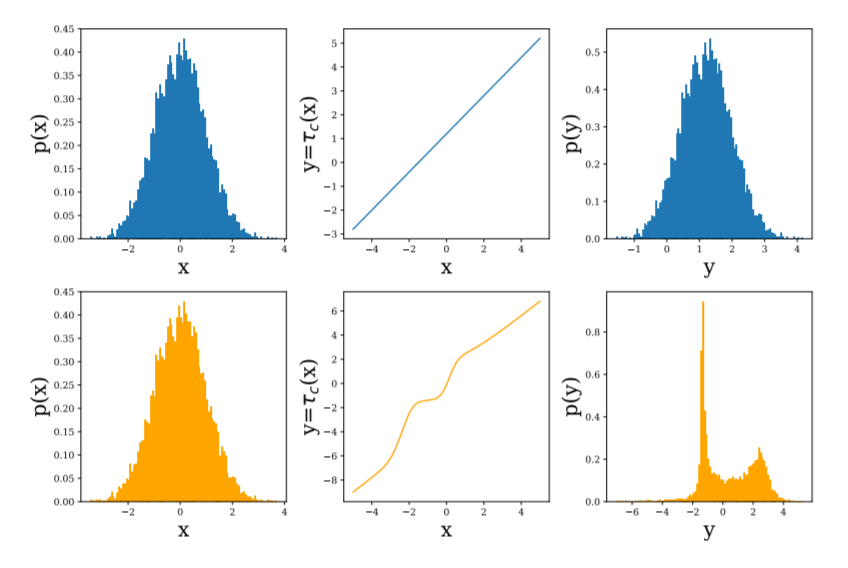
\includegraphics[width=0.6\textwidth]{Figures/naf.png}
            \vfill
            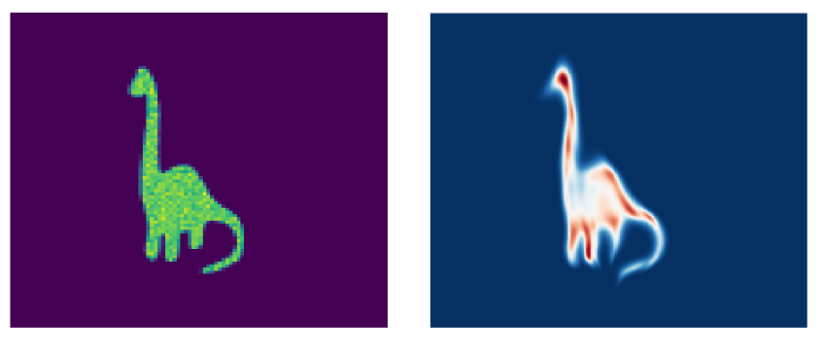
\includegraphics[width=0.3\textwidth]{Figures/dino.png}
        \end{center}
    \end{example}

    \framebreak

    \begin{example}[Masked autoregressive flows, MAF]
        \[
            y_i = \sigma(x_{1:i-1}) x_i + \mu(x_{1:i-1})
        \]
        \begin{center}
            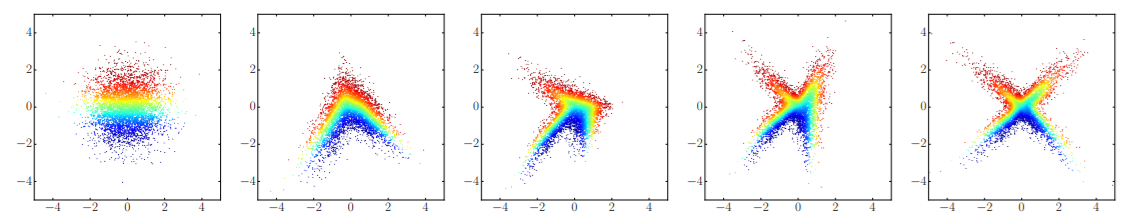
\includegraphics[width=0.8\textwidth]{Figures/nf-example.png}
        \end{center}
    \end{example}

    % TODO: show the tails are the same before and after this transform,
    % dinosaur is impresive but looks just like circle in the tails
\end{frame}

\begin{frame}[allowframebreaks]
    \frametitle{Beyond sub-Gaussians}

    \begin{theorem}[Wainwright ``High-dimensional statistics'' 2019]
        Let $X$ be $\sigma$-sub-Gaussian and $f$ be $L$-Lipschitz.
        Then $f(X) - \EE f(X)$ is $L$-sub-Gaussian.
    \end{theorem}

    \textbf{Observation}: Gaussian base distributions are pervasive!
    \begin{center}
        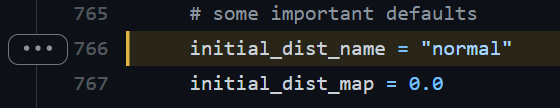
\includegraphics[width=0.45\textwidth]{Figures/pymc-normal.png}
        \footnote{https://github.com/pymc-devs/pymc3/blob/d7172c0a1a76301031d1b3b411d00643c416a0c4/pymc3/variational/opvi.py\#L766}
        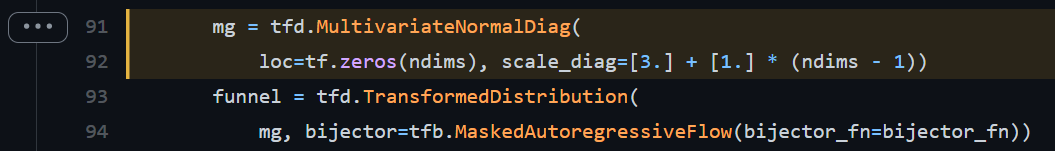
\includegraphics[width=0.45\textwidth]{Figures/tfp-normal.png}
        \footnote{https://github.com/tensorflow/probability/blob/22947dc575778318b660303129ee39c2a870e5a9/spinoffs/inference\_gym/inference\_gym/targets/neals\_funnel.py\#L91-L92}
        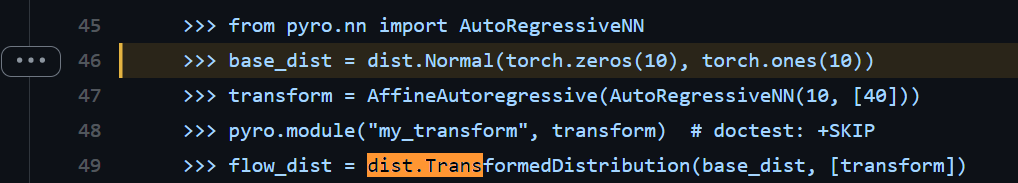
\includegraphics[width=0.45\textwidth]{Figures/pyro-normal.png}
        \footnote{https://github.com/pyro-ppl/pyro/blob/d7687ae0f738bd81a792dabbb18a53c0fce73765/pyro/distributions/transforms/affine\_autoregressive.py\#L46}
    \end{center}

    \textbf{Observation}: Many $f^W$ used in practice are Lipschitz!

    \begin{center}
        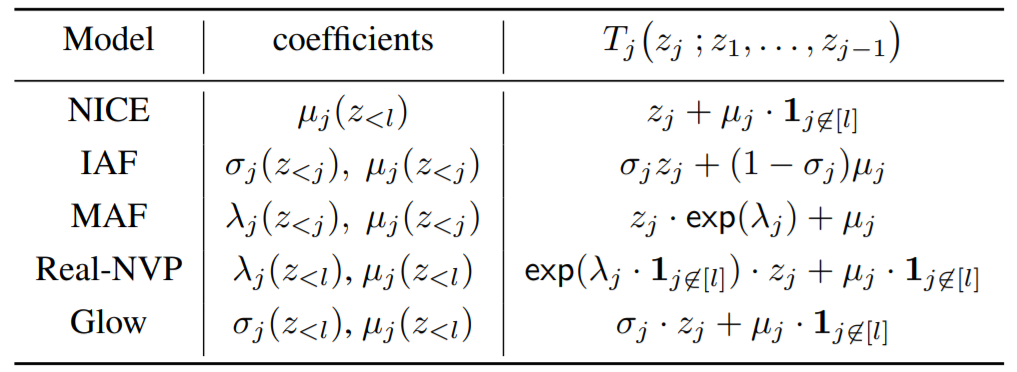
\includegraphics[width=0.6\textwidth]{Figures/jaini-table-1.png}
        \footnote{https://arxiv.org/pdf/1907.04481.pdf}
    \end{center}

    \begin{definition}[Classification of tails]
        \begin{itemize}
            \item Exponential-type: $X \in \cE_\alpha^p$ means $\PP(X \geq x) = \cO(e^{-\alpha x^p})$
            \item Logarithmic-type: $X \in \cL^p_\alpha$ means $\PP(X \geq x) = \cO(e^{-\alpha (\log x)^p})$
        \end{itemize}
    \end{definition}

    \begin{example}
        \begin{itemize}
            \item $\cE_\alpha^2$ sub-Gaussians
            \item $\cE_\alpha^1$ sub-Exponentials
            \item $\cL^1_\alpha$ regularly varying (power law)
                  \begin{itemize}
                      \item $\text{StudentT}(\nu) \in \cL^1_\nu$
                      \item $\text{Cauchy} \in \cL^1_1$
                  \end{itemize}
        \end{itemize}
    \end{example}

    \framebreak

    \textbf{Assumption 1}: $\lambda_j$ and $\sigma_j$ are bounded and $\mu_j$ is Lipschitz,

    \begin{theorem}[LHM, 2021]
        Under Assumption 1,
        the distribution classes $\cup_{\beta \in \RR} \cE_{\beta}^p$
        and $\cL^p_\alpha$ (with $p,\alpha \in \RR_+$) are closed
        under every flow transformation in Table 1.
    \end{theorem}

    \begin{theorem}[LHM, 2021]
        There does not exist a polynomial map between $\cL$ and $\cE$.
    \end{theorem}
    % $Y = X^k$, $\PP(Y \geq x) = \PP(X \geq x^{1/k}) = e^{-\alpha x^{p/k}} = \sum_l \frac{(-\alpha x^{lp/k})}{l!}$
    % is not asymptotically bounded by any polynomial.
\end{frame}

\begin{frame}
    \frametitle{Tail-adaptive flows (TAFs)}
    \begin{definition}
        \begin{align*}
            \cQ_{TAF} & = \left\{
            \left(f^W_\ast \left(\prod_{i=1}^d \text{StudentT}(\nu)\right)\right):
            \nu \in \RR_+, W \in \RR^{\text{\# NF params}}
            \right\}
        \end{align*}
    \end{definition}

    \begin{center}
        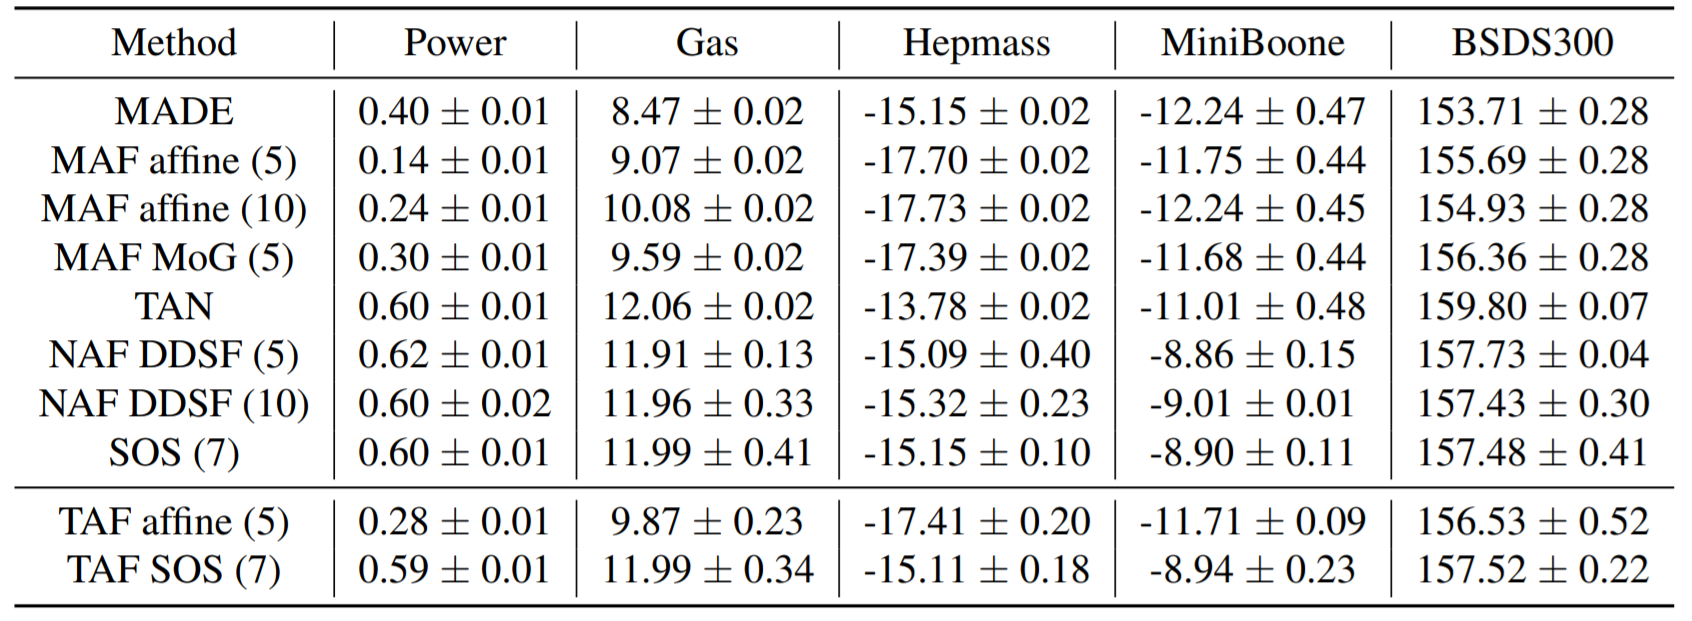
\includegraphics[width=1.0\textwidth]{Figures/taf-table.png}
        \footnote{Jaini, Priyank, et al. ``Tails of Lipschitz Triangular Flows.'' ICML 2020}
    \end{center}
\end{frame}

\begin{frame}
    \frametitle{Multivariate heavy-tails}

    \textbf{Prior work} (Jaini, 2020): $X \in \RR^d$ is heavy-tailed iff $\|X\|$ is,
    develop theory for elliptical distributions
    $\vec{X} \overset{d}{=} \vec{\mu} + R \matr{A} \matr{U}^{(d)}$.

    \textbf{Problem 1}: TAF's $\prod_1^d \text{StudentT}(\nu)$ is not elliptical
    \begin{center}
        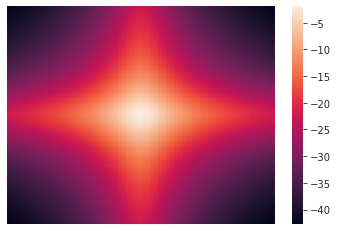
\includegraphics[width=0.4\textwidth]{../Figures/studentt-product.png}
    \end{center}

    \textbf{Problem 2}: Tail parameter $\nu$ is the same in every direction!
\end{frame}

\begin{frame}
    \frametitle{Direction-dependent tail parameters}

    \textbf{Root cause}: $\sup_{v \in \cS^{d-1}} \braket{v,X} = \|X\|_2$, so
    scalar tail parameter is an upper bound.

    \begin{definition}
        The \emph{tail parameter function}
        for a fat-tailed random variable $X \in \RR^d$
        \begin{align*}
            \alpha : \cS^{d-1} & \to \RR_+                                                                      \\
            v                  & \mapsto \limsup_{r\to\infty} \frac{\log\mathbb{P}(\|\braket{v,X}\|>r)}{\log r}
        \end{align*}
    \end{definition}

    \begin{example}
        Elliptical distributions are \emph{tail isotropic} i.e. $\alpha(v) \equiv c$ is constant.
    \end{example}

    \begin{proposition}[LHM, 2021]
        Let $\mu$ be elliptical or $\prod_1^d \text{StudentT}(\nu)$
        and suppose $f^W$ is invertible and satisfies Assumption 1.
        Then $f^W_* \mu$ is tail isotropic with $\alpha \equiv \nu$.
    \end{proposition}
\end{frame}

\begin{frame}
    \frametitle{Standard basis tail parameters}

    $\alpha(\cdot)$ difficult to work with; need finite-dimensional parameterization which
    still permits tail anisotropy.

    \vspace{.5cm}

    \textbf{Key observation}: multivariate distributions oftentimes obtained from concatenation
    (blocked Metropolis-Hastings, Hamiltonian Monte-Carlo) $\implies$ tails are axis-aligned.

    \vspace{.5cm}


    \begin{definition}
        The \emph{standard basis tail parameters} are $\{\alpha_i \coloneqq \alpha(v_i) : i \in [d]\}$
    \end{definition}

    % \begin{center}
    %     \includegraphics[width=0.7\textwidth]{../Figures/mv-tail-param-sketch.png}
    % \end{center}

\end{frame}

\begin{frame}
    \frametitle{Fat-tailed variational inference (FTVI)}

    \begin{definition}
        \begin{align*}
            \cQ_{FTVI} & = \left\{
            \left(f^W_\ast \left(\prod_{i=1}^d \text{StudentT}(\nu_i)\right)\right):
            \nu \in \RR_+^d, W \in \RR^{\text{\# NF params}}
            \right\}
        \end{align*}
    \end{definition}

    \begin{remark}
        Let $\mu = \prod_1^d \text{StudentT}(\nu_i)$
        and suppose $f^W$ is invertible and satisfies Assumption 1.
        Then $f^W_* \mu$ can be tail anisotropic.
        % Moreover, its standard basis tail parameters are equal
        % (up to permutation) to those for $\mu$.
    \end{remark}

    % \begin{proof}
    %     asymptotics to saturate scale, only $z_j$ left.
    % \end{proof}
\end{frame}

\begin{frame}
    \frametitle{Results: fat-tailed pancake}

    \begin{center}
        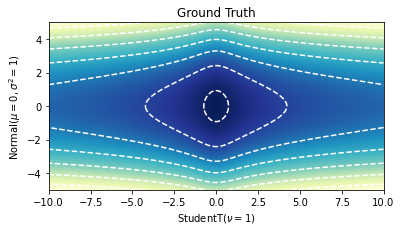
\includegraphics[width=0.48\textwidth]{../Figures/pancake-truth.png}
        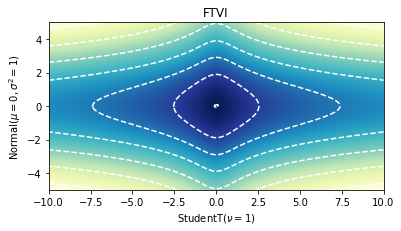
\includegraphics[width=0.48\textwidth]{../Figures/pancake-ftvi.png}
        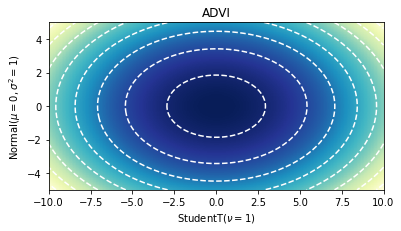
\includegraphics[width=0.48\textwidth]{../Figures/pancake-advi.png}
        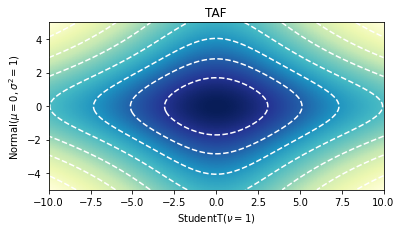
\includegraphics[width=0.48\textwidth]{../Figures/pancake-taf.png}
    \end{center}
\end{frame}

\begin{frame}[fragile]
    \frametitle{Results: gamma scale mixture}

    \begin{lstlisting}
scale = InvGamma(1/2, 1/2)
truth = scale.sqrt() * Normal(0, 1)
    \end{lstlisting}

    \begin{center}
        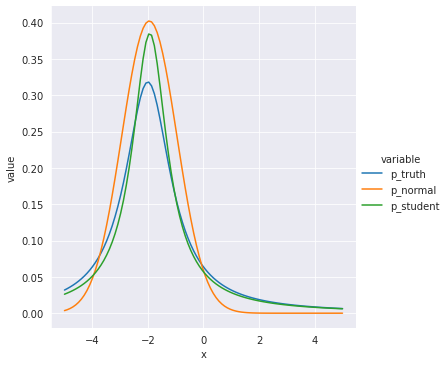
\includegraphics[width=0.49\textwidth]{../Figures/cauchy_normal_student.png}
        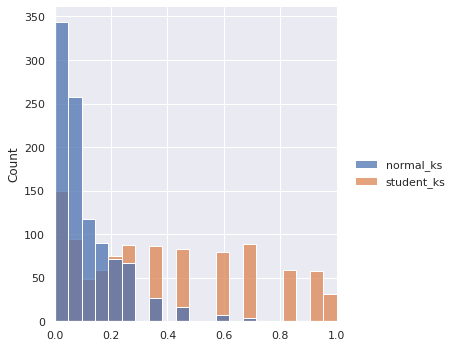
\includegraphics[width=0.49\textwidth]{../Figures/cauchy_ks.png}
    \end{center}
\end{frame}


\begin{frame}
    \frametitle{Results: eight-schools}

    % Flows improve over ADVI, FTVI flows improve over Gaussian base,
    % depth matters

    \begin{center}
        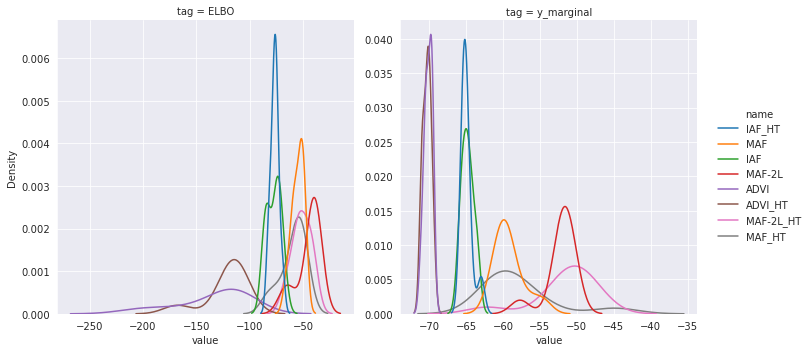
\includegraphics[width=0.7\textwidth]{../Figures/eight_schools.png}
        \begin{tabular}{rcc}
            \toprule
                      & ELBO                & $\log P(y)$       \\
            \midrule
            ADVI      & -193.86 $\pm$ 33.50 & -70.11 $\pm$ 0.52 \\
            ADVI-HT   & -121.54 $\pm$ 19.59 & -70.29 $\pm$ 0.54 \\
            MAF       & -55.06 $\pm$ 5.46   & -59.14 $\pm$ 1.99 \\
            MAF-HT    & -59.63 $\pm$ 6.74   & -57.84 $\pm$ 4.97 \\
            MAF-2L    & -45.01 $\pm$ 11.02  & -52.19 $\pm$ 2.06 \\
            MAF-2L-HT & -51.67 $\pm$ 8.72   & -51.53 $\pm$ 4.23 \\
            % IAF       & -77.67 $\pm$ 6.47   & -64.79 $\pm$ 0.80 \\
            % IAF-HT    & -76.67 $\pm$ 3.71   & -64.91 $\pm$ 0.76 \\
            \bottomrule
        \end{tabular}
    \end{center}
\end{frame}

\begin{frame}
    \frametitle{Tail index algebra}
    \begin{itemize}
        \item Many of previous proofs rely on a few common lemmas, extract into
              an easy-to-use algebra
        \item Enables a priori tail index estimation without samples
              (quick and dirty upper bounding, initializing $\nu$ for VI)
        \item Handles addition, multiplication, division, concatenation, exp/log, Lipschitz functions
              % concatenation's min goes against tail parameter function's anisotropy idea
        \item Conditioning: conditional asymptotically equivalent to joint
    \end{itemize}
\end{frame}


\end{document}